This chapter presents an IMP solution which solves issues of OZG identity management described in chapter 3 through integration of the IMP system described in section 2.2 into the OZG system architecture described in section 2.4. Focus of this solution is to not be invasive into the existing system architecture: Few existing system components should have to be modified and the existing operation of the system should not be disrupted. This enables the introduction of IMP as an additional but optional way of accessing OZG services with improved usability.

The integration of the IMP system takes place on three layers:

\begin{center}
    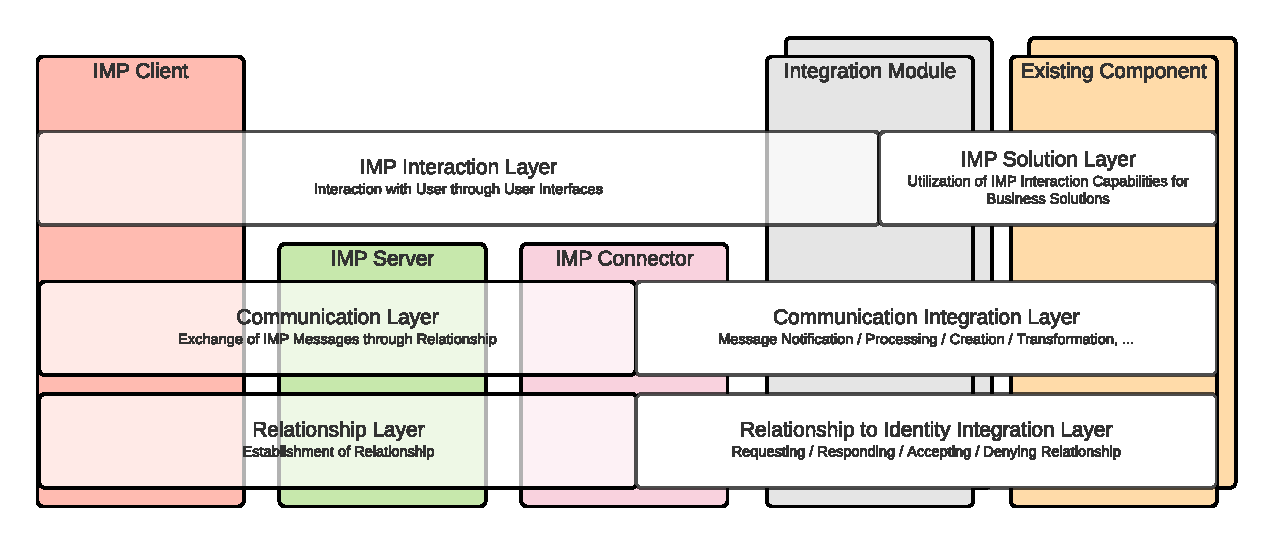
\includegraphics[scale=0.6]{Diagrams/Integration Architecture 1/IMP Layer Diagram Integration.pdf}
\end{center}

\paragraph{IMP Solution Layer} 
The purpose of the integration on the IMP solution layer is to take advantage of new interaction capabilities with the user through the IMP system. The integration evaluates possibilities of using relationships and IMP messages to improve OZG services, defines what the purpose of each message and relationship type is and how they should be handled by client and service provider. For example relationship templates can be defined and new message types can be created with corresponding new user interfaces in the IMP client.

\paragraph{Technological Integration} The technological integration on the "Communication Integration" layer and the "Relationship To Identity Integration" layer describes how an integration system can enable the existing system architecture to implement the IMP solution described in the "IMP Solution" layer.

\section{IMP Solution Integration}

\subfile{10-imp_solution_integration}

\section{Technological Integration}

\subfile{11-technological_integration}

\section{Solution Evaluation}

\begin{itemize}
    \item Messaging enables existing system architecture to process events
\end{itemize}

The described IMP solution combines the existing identity management solution of the OZG with new IMP services, increasing usability trough a non-invasive integration while compromising on data protection.

The IMP solution enables users to manage their OZG user profile as one of multiple IMP relationships which enables him to keep an overview of shared attributes and how they are being processed. The user can update personal information and receive notifications in one place. Using the IMP client for authentication, the user wont need to remember user password for his user profile.

For the service provider, the integration architecture is non-invasive, as only two system components are required to connect to a messaging adapter and the existing operation of the system architecture is not disturbed. As a result of the modular messaging approach, the integration can easily be expanded with new features by adding new modules.

However, the simplified integration comes at a cost for the user. Most of the basic use case as well as most personal information is still being processed by the administration portals. This remains to be a data protection issue. As the administration portal only establishes one type of relationship for accessing all necessary personal information, differentiation in processing the individual attributes is difficult. The user also is required to approve to a very general request for sharing attributes: "Create user profile". Further legitimisation for processing personal information e.g the individual administrative services remain to be hidden from the IMP client.

In the future, the described IMP solution can eventually replace interoperable user profiles. If every administration portal integrates the IMP solution and establishes its own IMP relationship with users, user profiles will no longer need to be interoperable as the user can easily manage the individual relationships trough one IMP client.

\begin{itemize}
    \item Can eventually replace interoperable user profiles by each administration portal only using IMP and user profiles "behind the scenes"
    \item Can eventually replace user profiles by using relationships to apply for services
\end{itemize}